%\chapter{Vocal Accommodation for Conversation Intelligence}
\chapter{Vocal Accommodation in Real-World Sales Calls}
\label{chap:conv_analysis}

\lettrine{C}{onversation} intelligence deals with the analysis and management of data accumulated during an interaction, e.g., to draw conclusion about the interlocutors.
This chapter includes examples of vocal accommodation used as a mean for analyzing patterns, structures, and behaviors in different interaction setups.

\pagebreak

\section{Conversation intelligence}
\label{sec:conversation_intelligence}

%\Acf{ci}, also known as \textit{conversation IQ} (\aca{ci}), is\ldots

\citet{Glaser2016conversational}
\citet{SilberVarod2018human}

\section{Speaker roles and influences in sales calls}
\label{sec:speaker_roles_and_influences_in_sales_calls}

\section{Capturing different behaviors with \acs{crqa}}
\label{sec:capturing_behaviors}

Linear methods for measuring accommodation rely on the chronological, turn-by-turn order of the interaction.
These methods are limited to detection of local phenomena evolving gradually across adjacent turns.
Non-linear methods, contrarily, are not dependent on the chronological order of the interaction's turn and can therefore find long-term, more distant relations between the speakers with respect to the target feature.
For instance, that an accommodation process (or generally closer values) occurred at some point in the beginning and continued at a later time, or that there was a periodic pattern of convergence and divergence throughout the interaction.
Such phenomena point to more general, conversation-level properties that do not rely on the unfolding chronological order of the turns.
This is especially useful for long interaction, where a more general view may be insightful.
Non-linear analysis methods for time series include, for example, noise reduction and non-linear prediction.
We utilize here another method that uses phase-space embedding, which describes temporal evolution of trajectories of a dynamic system by projecting their embedding onto some common space.

\todo[inline]{find 1-2 more examples of non-linear methods, and say that here we present CRQA}

\subsection[\Acl{crqa} for measuring accommodation]{\Acl{crqa}}
\label{subsec:crqa}

\begin{figure}[t]
	\centering
	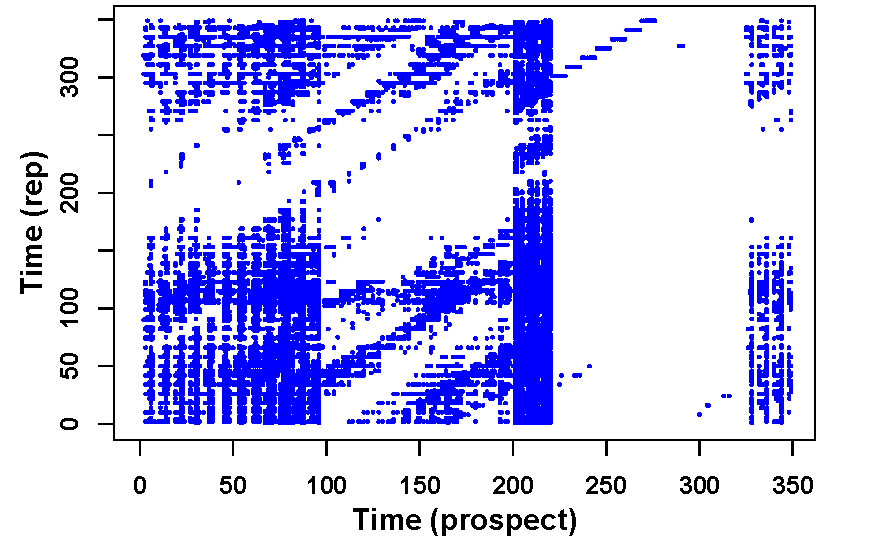
\includegraphics[width=\linewidth]{crqa_plot_115993376241473405}
	\caption
	[\acs{crqa} analysis of pitch in a sales call]
	{A recurrence plot generated for one of the analyzed conversations.
		The y-axis marks the conversation timeline, in time stamp, of the \ac{ae}, and the x-axis of the prospect.
		Each blue dot represents a co-visitation of a similar state.
		Blue dots forming an diagonal line indicate sustained recurrence between the two speakers (see description of NRLINE in \cref{subsubsec:output_values} for details).
		Note that the time stamps on the axes are not the slices, but the embedded call time. 
		For example, the diagonal structures between time stamps 100 and 200 of the x-axis show such lasting recurrence.
		Diagonal lines above the \acl{los} (\acs{los}; the central diagonal line) indicate that the speaker on the y-axis leads the x-axis, and vice versa for lines below the \ac{los}.
		The blank area between time stamps 220 and 330 of the x-axis point to a portion of the call where the speakers were more distant from each other.}
	\label{fig:crqa_plot}
	\todo[inline]{make the plot square, to make it clearer that the times have the same length}
\end{figure}

In the studies present here, the target features are either evaluated when detected or sampled in defined intervals using a dedicated system for accommodation analysis \citep{Raveh2018Specom}.
\todo{make sure there is more explanation about how this is done where the experiments are described}
Furthermore, these values are extracted in chronological order, and thus produce sequences of discrete-time data.
Based on these characteristics, they can be treated as \emph{time series}.
Due to the nature of these features (and perhaps any spontaneous, interactive linguistic feature), the resulted time series can be assumed to be non-seasonal and non-stationary.
This recognition as time series opens new methodological possibilities for examining the evolution of these features and their realizations by different speakers in an interaction over time.
Such methods include, among others, autocorrelation for examining serial dependency and forecasting for transferring information about the time series across time.
These methods can extend upon others in analyzing accommodation, with the advantage of offering more dynamic approach rather than the sequential methods usually used.
One such analysis method is \acf{crqa}, which provides insights on the time series across an entire time span.
This is done by comparing delayed instances of the phase-space trajectories of time series.
This allows finding more general patterns in the time series characteristics and how they interact.
It is especially suitable for studying accommodation and related phenomena, as it detect times in which the time series are more similar and can mathematically show which of this time series led the changes or whether the changes were done in synchrony.
Therefore, \ac{crqa} can be use to objectively quantify and describe accommodation between speakers.
\crefrange{subsubsec:detecting_recurrence}{subsubsec:parameters_crqa} explain how \ac{crqa} works, how its output can be interpreted, and how it is used in the studies presented here.

\subsubsection{Detecting recurrence}
\label{subsubsec:detecting_recurrence}

\Ac{rqa} is a method of non-linear data analysis that quantifies the number and duration of recurrences of a dynamical system presented by its state space trajectory, which is typically the realization of a sampled time series
It was developed by \citet{Zbilut1992embeddings} and was extended by \citet{Webber2005recurrence,Marwan2002cross}.
A \emph{recurrence} (also, \emph{re-visitation}) is a time in which the trajectory returns to a state (or a similar-enough state) it has visited before.
Recurrence can therefore be defined as the binary function

\begin{equation}
\label{eq:recurrence}
R_{i,j} =
\begin{cases}
1,	&	\text{if} \quad \lVert \vec{x}(i)-\vec{x}(j) \rVert \leq \varepsilon \\
0,	&	\text{otherwise} \\
\end{cases},
\end{equation}
%
where $i$ and $j$ are x-axis and y-axis coordinates in the plot, respectively, and $\varepsilon$ defines some threshold distance between cross-trajectory point pairs to consider them similar (see explanation about the \emph{radius} parameter below).
In a plot, $R_{i,j}$ points are colored equal if their value is 1 or stay white otherwise.

\Ac{crqa} is an extension of \ac{rqa} with recurrence quantification of two different time series rather than a single one.
As such, \ac{crqa} is a quantification technique for non-linear dynamical systems that describes when and to what extent recurrences (or \emph{co-visitations}) can be found in two time series.
These quantification techniques are based on \emph{recurrence plots} that for each moment $i$ in time show the times at which a phase space trajectory visits roughly the same area in the phase space as at time $i$.
Ultimately, a recurrence plot is a graph of $\vec{x}(i) \approx \vec{x}(j)$, showing $i$ on the x-axis and $j$ on the y-axis, where $\vec{x}$ is a phase space trajectory (see example in \cref{fig:crqa_plot}).
\todo[inline]{take one of the RPs from the website and add the LoS (and other diagonals) to it to provide more detailed visualization}
Each colored point in the plot represents a time where the time series were close to each other based on the definition in \cref{eq:recurrence}.
The main diagonal of the plot is called the \acf{los}.
A high number of recurrences along this line indicates synchrony between the time series (many points in time with similar values).
However, diagonal recurrence lines can be formed above and below the \ac{los}.
Such diagonals, especially longer ones, represent delayed (lagged) synchrony between the time series and can be used as an assessment of similarity between the processes.
In the context of accommodation, these diagonals imply an accommodative change led by one of the interlocutors.
If the diagonal stretches above the \ac{los}, the speaker plotted on the x-axis leads the accommodation, and vice versa.
The closer the diagonal is from the \ac{los}, the quicker the process occurred, i.e., the led speaker matched his behavior to the leading speaker in a shorter time.
Due to its ability to detect these similarities non-linearly, \ac{crqa} can be utilized to measure accommodation in the scope of entire conversations rather than taking only neighboring turns into account \citep[cf.][]{Levitan2013entrainment}.
For instance, it has already been used to describe behavior in conversations \citep{Duran2017conversing} and to measure conversational entrainment for assessing speech pathology \citep{Borrie2019syncing}.

\subsubsection{Parameter tuning}
\label{subsubsec:parameters_crqa}

\Ac{crqa} requires three parameters to run:

\begin{enumerate}
	\item \textbf{Delay} -- estimates the temporal shift required to make the two time series maximally aligned.
	It is measured by the same time unit as the time series, in the presented studies, a slice (see \putref{reference to where feature extraction is described}).
	
	\item \textbf{Embedding dimensions} -- are the number of dimensions into which the data points are embedded.
	These dimensions are delayed copies of the original time series $S(t)$ created by adding a lag $k$ to them.
	Typically, multiple lags are considered, which create the dimensions of embedding $S(t + nk)$.
	
	\item \textbf{Radius} -- determines the margin within which two data points are considered a recurrent instance.
	Distances between the data points are measured in the embedded space defined by embedding dimensions, using the same unit used for measuring the values of the time series.
\end{enumerate}
%
These parameters are a key aspect in \ac{crqa} and how they are set is crucial for its outcome.
However, there is no standard way for optimizing these parameters, especially due to the fact that they depend on the nature and characteristics of the data, although some best-practice guidelines are suggested by \citet{Coco2014crqa-r},

A method similar to the one presented by \citet{Marwan2007recurrence} was utilized for the studies presented here.
The delay parameter was determined by finding the lag that minimizes the mutual information between the two time series.
This provides a delay that is not too short to miss the different distributions, but also not too long to lose the dependency between the time series.
The lag with the \emph{lowest} mutual information was selected, regardless of when the values started to level off.
Subsequently, the number of embedding dimensions was obtained using false nearest neighbors \citep{Kennel1992determining}.
This algorithm determines the minimum embedding dimension necessary to reconstruct the state space of a dynamical system with time delay embedding \citep{Abarbanel1993local}.
We used a neighborhood diameter equal to the standard deviation of the time series and set a limit of 20 embedding dimensions (which was never reached).
\crefrange{fig:ami}{fig:false_nn} show examples of mutual information and false nearest neighbours optimizations.

\begin{figure}[H]
	\centering
	\begin{minipage}{.45\linewidth}
		\centering
		\includegraphics[width=\linewidth]{ami}
		\caption
		[Average mutual information of time series as function of lag]
		{The average mutual information of the time series values as a function of the lags considered.
			The x-axis shows the considered lags and the y-axis the mutual information index (AMI) in bits.}
		\label{fig:ami}
	\end{minipage}%
	\hfill
	\begin{minipage}{.45\linewidth}
		\centering
		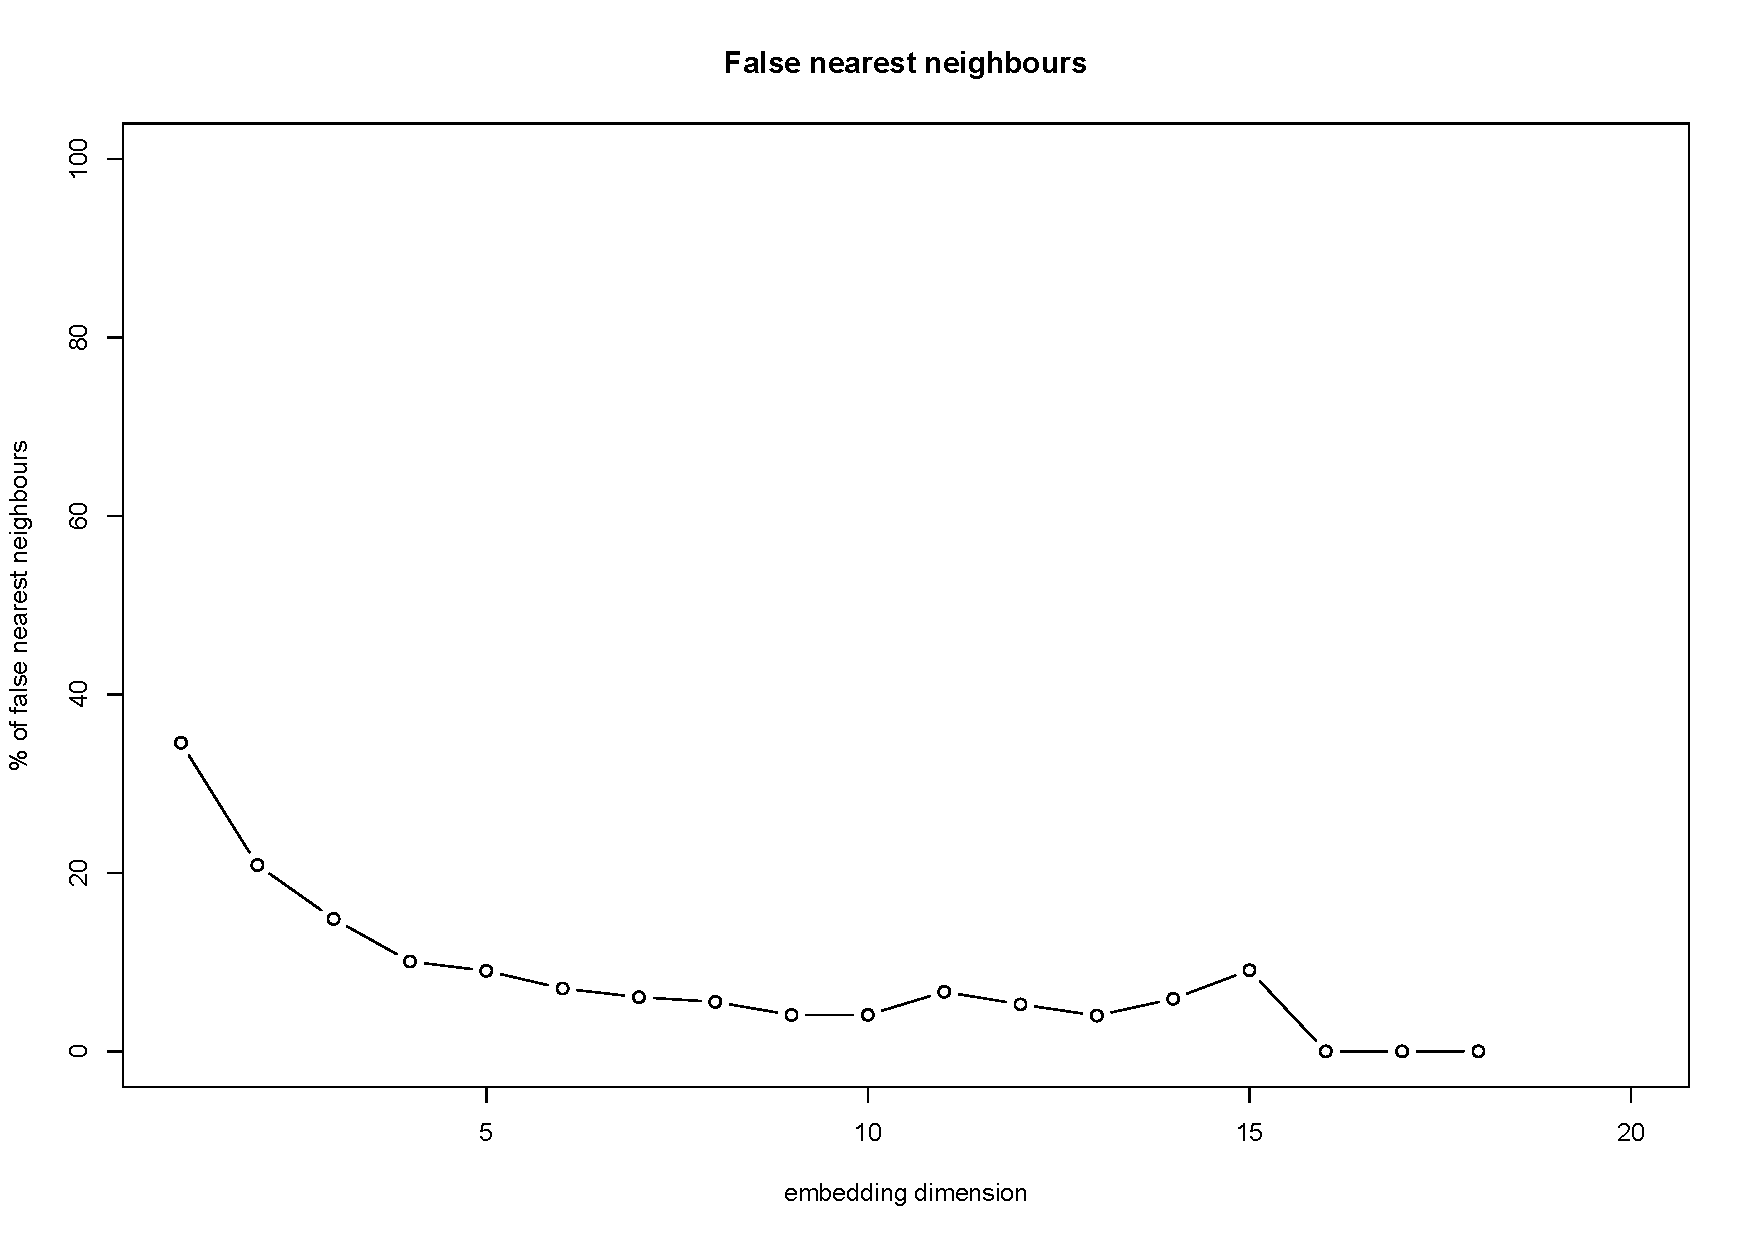
\includegraphics[width=\linewidth]{false_NN}
		\caption
		[Embedded dimensions optimization]
		{False nearest neighbours percentage as a function of the number of embedded dimensions.
			The x-axis show the considered numbers of embedded dimensions and the y-axis the percentage of false nearest neighbours.}
		\label{fig:false_nn}
	\end{minipage}	
\end{figure}

Then, the radius was calculated in two steps (see \cref{alg:radius_opt}).
First, the goal \ac{rr} and a list of potential radii were set.
Here, the goal \ac{rr} was set to \SI{10}{\percent}, which is relatively high (e.g., compared to \SIrange{2}{5}{\percent} in \citet{Coco2014crqa-r}).
Setting the goal \ac{rr} to a higher value results in a stricter optimization that will reward closer recurrences in the analysis.
The potential radii were generated by evenly spreading 20 candidates from 0 to the maximum value that occurs in the time series.
After that, each radius, along with the already optimized delay and embedding dimensions, was used to perform a \ac{crqa}.
This step also introduced a stricter policy, as only lines longer than \SI{1}{\percent} of the length of the time series were counted, as opposed to the typical setup that considers lines of any length.
With an average length of \SI{37.5}{minutes}, this means that lines longer than 11 time units, compared to the a typical setup with the minimal length of two time units (e.g., as done by \citet{Borrie2019syncing}).
This ensured that only long-term recurrences were taken into account, and filtered out shorter, possibly more random effects.
% note: calculated by multiplying 37.5 minutes * 60 to get seconds. then divide by 2 since each time unit (slice) was 2 seconds and again divide by 100 to get one percent of it.
Finally, the candidate radius that results in the smallest absolute distance from the goal \ac{rr} was taken as the optimized radius to perform \ac{crqa}.
The radius optimization is described in \cref{alg:radius_opt}
The optimization processes of all three parameters were done for each interaction separately.

\begin{algorithm}[t]
	\caption{\acs{crqa} radius optimization}
	\label{alg:radius_opt}
	%	\eqname{\acs{crqa} radius optimization algorithm}
	\algorithmcaption{\emph{The higher $n$ is (\cref{line:num_cand}), the higher the chance of a \ac{rr} close to the defined \emph{desired RR}.
			Also note that since \ac{rr} represents percentage of values in the recurrence plot, 100 is its highest possible value.
			Therefore, and since the radii in $R$ are traversed in increasing order, the search stops if this value is achieved (\cref{line:break_at_rr_100}).
			As explained in the text, in the presented studies $n = 20$ and $desiredRR = 10$ (see \citet{Coco2014crqa-r}).}}
	\DontPrintSemicolon
	\SetKwInOut{Input}{Inputs}
	\SetKwInOut{Output}{Output}
	
	\Input{\underline{$desiredRR$} -- the desired approximated \ac{rr} value\newline
		\underline{$optDelay$} -- the optimized delay\newline
		\underline{$optEmbedim$} -- the optimized embedded dimensions\newline
		\underline{$TS$} -- all values from both time series}
	\Output{radius producing \ac{rr} value closest to the defined desired \ac{rr}\newline}
	
	$n \gets$ number of radius candidates \label{line:num_cand}\;
	$R \gets \{r_i, \ldots, r_n\} : r_1 = 0, r_n = \max(TS)$\;
	$\forall r \in R : \lvert r_i - r_{i-1} \rvert = \lvert r_{i+1} - r_i \rvert$ \tcp*{evenly spread candidates}
	
	$candR \gets \varnothing$\;
	\ForEach{$r \in R$}{
		$currRR = crqa(ts_1, ts_2, optDelay, optEmbedim, \ldots\footnotemark).RR$ \tcp*{RR with candidate}
		$candR = candR \cup currRR$\;
		\uIf{$currRR = 100$}
		{\emph{break} \label{line:break_at_rr_100} \tcp*{\ac{rr} cannot be higher than 100}
		}
	}
	$optRadius = \displaystyle\argmin_{r \in R}(\lvert candR_r - desiredRR \rvert)$\;
\end{algorithm}
\footnotetext{As calculated by the \ac{crqa} package for R \citep{Coco2014crqa-r} with the additional arguments (unlisted in the algorithm itself) \emph{rescale=0, normalize=0, minvertline=length(ts1) / 100, mindiagline=length(ts1) / 100,} and \emph{tw=0}.}
\todo{make sure algorithm block is on same page with its footnote}

\subsubsection{Output values}
\label{subsubsec:output_values}

As detailed in \citet{Marwan2007recurrence}\footnote{and see summary with additional measures in \url{http://www.recurrence-plot.tk/rqa.php}}, several measures can be computed based on a recurrence plot.
Some measurements deal with the \ac{los} and other diagonals and others with vertical/horizontal lines.
Below are the definitions of some \ac{crqa} measurements used in this work.
For simplicity, in the descriptions it is assumed that the time series lengths are equal, so that $N_i=N_j=N$.

\begin{description}
	\item[\Acf{rr}] The percentage of recurrent points in the plot, i.e., the percentage of similar values between the two time series out of all the values.
	This corresponds to the correlation sum and defined as
	
	\begin{equation}
	\label{eq:rr}
	RR = \frac{1}{N^2} \sum_{i=1}^{N_i} \sum_{j=1}^{N_j} R_{i,j}.
	\end{equation}
	%	\eqname{CRQA measure definitions: RR, DET, L, maxL, ENTR, and rENTR}
	%
	Note that the lengths of the time series ($N_i$ and $N_j$) are often -- but not necessarily -- equal
	
	\item[Determinism (DET)] The percentage of recurrences forming diagonal lines in the recurrence plot given a minimal length threshold $l_{\min}$.
	\begin{equation}
	\label{eq:det}
	DET = \frac{\sum_{l=l_{\min}}^{N} l P(l)}{\sum_{l=1}^N l P(l)},
	\end{equation}
	%
	where $l$ is the length of a line and $P(l)$ is the histogram of the lengths $l$ of the diagonal lines.
	Note that $l=1$ refers to lines of length 1, i.e., a single recurrence dot.	
	Similarly, $l=2$ are lines spanning over two time stamps (shortest length possible).
	This length is very forgiving in the context of accommodation, for such short lines can be formed arbitrarily and do not necessarily point to a meaningful accommodation process.
	Therefore, in the experiments presented here $l_{\min}$ was set to \SI{1}{\percent} of $N$.
	
	Another measure, Laminarity (LAM), can be calculated the same way, but for the vertical lines in the plot.
	In that case, a $v_{\min}$ would be defined and $P(v)$ would provide the histogram of vertical line lengths.
	
	\item[Number of lines (NRLINE)] The total number of lines formed in the recurrence plot $N_l$.
	This is the number of accommodation instances between the two speakers lasting at least $l_{\min}$ time stamps.
	Also referred to as \emph{sustained recurrence} by \citet{Borrie2019syncing}, defined as the amount of alignment between conversational partners, where higher sustained recurrence values indicate higher amounts of sustained accommodation.
	As explained in the description of the measure \emph{DET}, only lines of length $\frac{N}{100}$ and longer were taken into account in the studies presented here to exclude \enquote{arbitrarily formed} diagonals.
	
	\item[Maximal length (maxL)] The longest diagonal line in the plot, excluding the main diagonal.	
	This is the longest, uninterrupted time span accommodation between the speakers lasted.
	Higher value indicates a longer time span.
	The unit of this measure is the same as the axes of the plot (here, a representation of the conversation's turns).
	It is determined by
	
	\begin{equation}
	\label{eq:maxl}
	L_{max} = \max_{l} (\{l_i; \ i=1, \ldots, N_l\}).
	\end{equation}
	%
	The longest vertical line can be determined by traversing the vertical lines.
	
	\item[Average length (L)] the average length of the diagonal lines, i.e., the average total accommodation time between the speakers.
	Higher value indicates longer average individual accommodation periods during the interaction.
	This is calculated by
	
	\begin{equation}
	\label{eq:l}
	L = \frac{\sum_{l=l_{\min}}^N l P(l)}{\sum_{l=l_{\min}}^N P(l)}.
	\end{equation}
	%
	The average length of vertical lines, the trapping time (TT), is achieved in a similar way when using the same formula for the vertical line length and vertical line lengths histogram.
	
	
	\item[Entropy (ENTR)]The Shannon entropy of the probability distribution of the diagonal line lengths longer than the minimum length $l_{\min}$.
	Describes the variability of the amount of accommodation between the two speakers across the whole interaction.
	Higher value indicates more varied length of accommodation periods across the interaction.
	Shannon's entropy formula provides the value:
	
	\begin{equation}
	\label{eq:entr}
	ENTR = -\sum_{l=l_{min}}^{N} p(l) \ln p(l),
	\end{equation}
	%
	where $p(l)$ is the probability of length $l$ from the lengths probability distribution.
	\item[Normalized entropy (rENTR)] the entropy value normalized by the number of lines formed in the recurrent plot.
	This measure gives an idea how the speakers vary across multiple calls with different characteristics.
	
\end{description}

\todo[inline]{introduction to results}

Since multiple values are compared here, Bonferroni correction was applied, so that the overall error rate is \SI{0.05}{\percent}.
Therefore, for a single comparison to be significant, it must be lower than $\alpha = 0.007$.
The non-parametric two-sample Wilcoxon test \citep{Wilcoxon1945individual} was used to determine the significance levels.
\cref{tab:crqa_results} shows a summary of means and p-values of these outputs between failed and successful calls.
The \ac{rr} mean value is about 10 in all groups, which proves to be a suitable goal for optimizing the parameters (see \cref{subsec:crqa}).
Significant differences between failed and successful calls were found for the values DET, NRLINE, and rENTR.
The first two, along with their higher means for the failed calls, indicate more time-synchronized convergence in the failed calls.
The latter is harder to interpret, especially due to the similar means for successful and failed calls.
It therefore seems that the behavior in both cases is evenly predicted, but differently across calls.
One possible factor influencing these behaviors is related to the interlocutor leading the convergence, rather than the fact that it occurs at all.

\begin{table}[t]
	\caption{P-values of the two-sample Wilcoxon test comparing the \ac{crqa} output values between calls with success/fail outcome and their respective mean values.
		Significant values based on the adjusted p-value are set in bold.}
	\label{tab:crqa_results}
	\begin{tabularx}{\linewidth}{XSSSS}
		\toprule
		& {\thead{\acs{rr}}} & {\thead{DET}} & {\thead{NRLINE}}	& {\thead{maxL}} \\
		\midrule
		p 				& 0.9		& \bfseries $\ll$ 0.001	& \bfseries $\ll$ 0.001	& 0.7	\\
		mean success	& 10.1		& 2.2					& 84.0					& 31.3	\\
		mean fail		& 10.0		& 5.9					& 174.0					& 32.9	\\
		
		%			p (leaders)		& 0.7		& 0.1						& 0.05						& 0.18\\
		%			mean \acsp{ae}	& 10.0		& 6.1						& 186.7						& 35.2\\
		%			mean prospect	& 10.1		& 5.4						& 154.4						& 31.2\\
		\midrule
		& {\thead{L}} & {\thead{ENTR}} & {\thead{rENTR}} & \\
		\midrule
		p 				& 0.07		& 0.1		& \bfseries 0.0058	& \\
		mean success	& 17.8		& 1.4		& 0.8				& \\
		mean fail		& 15.3		& 1.5		& 0.8				& \\
		
		%			p (leaders)		& 0.9		& 0.07		& 0.55					& {\qquad\qquad}\\
		%			mean \acsp{ae}	& 15.2		& 1.5		& 0.8					& {\qquad\qquad}\\
		%			mean prospect	& 15.7		& 1.4		& 0.8					& {\qquad\qquad}\\
		\bottomrule	
	\end{tabularx}
\end{table}

To shed more light on the role of a leading partner, we used \acl{cc} to determine which interlocutor leads the change in behavior.
As shown in \cref{fig:crqa_plot}, \ac{crqa} reports at which points in time the speakers were more inclined to be closer to each other.
As an extension, \acl{cc} finds the degree to which two time series are synchronized at different points in time.
For each such point, called \emph{lag}, the \acl{cc} function evaluates the correlation between the time series.
By iterating over a set of time points, the shift needed to make the time series maximally correlated can be found.
If this lag is positive, the first time series needs to be shifted forward to achieve maximal correlation, and vice versa.
In the context of convergence, \ac{cc} calculates the direction of the shift, which indicates which speaker leads the change.
The \acl{cc} function was not limited to a specific range of shifts, so that all possible lags were examined.
The lag associated with the maximal correlation -- and only it -- was used to determine the leader.
Since these calls have a typical structure, it is also interesting to see at which point of the conversation the maximal correlation occurs.
\cref{fig:barplot_conv_leaders} shows the time, in percent, in which the maximal correlation occurred for \acp{ae} and prospects in successful and failed calls.
The difference between the lag position distribution of reps and prospects is significant, with a p-value of \num{0.0065} at $\alpha = 0.05$.
However, the differences between successful and failed calls within the leading speakers are not significant.
It is also evident that when the reps lead, they do so consistently at the very beginning of the conversation, all the more so in successful calls, whereas the prospects' lead varies much more and generally happens at a much later time.

\begin{figure}[t]
	\centering
	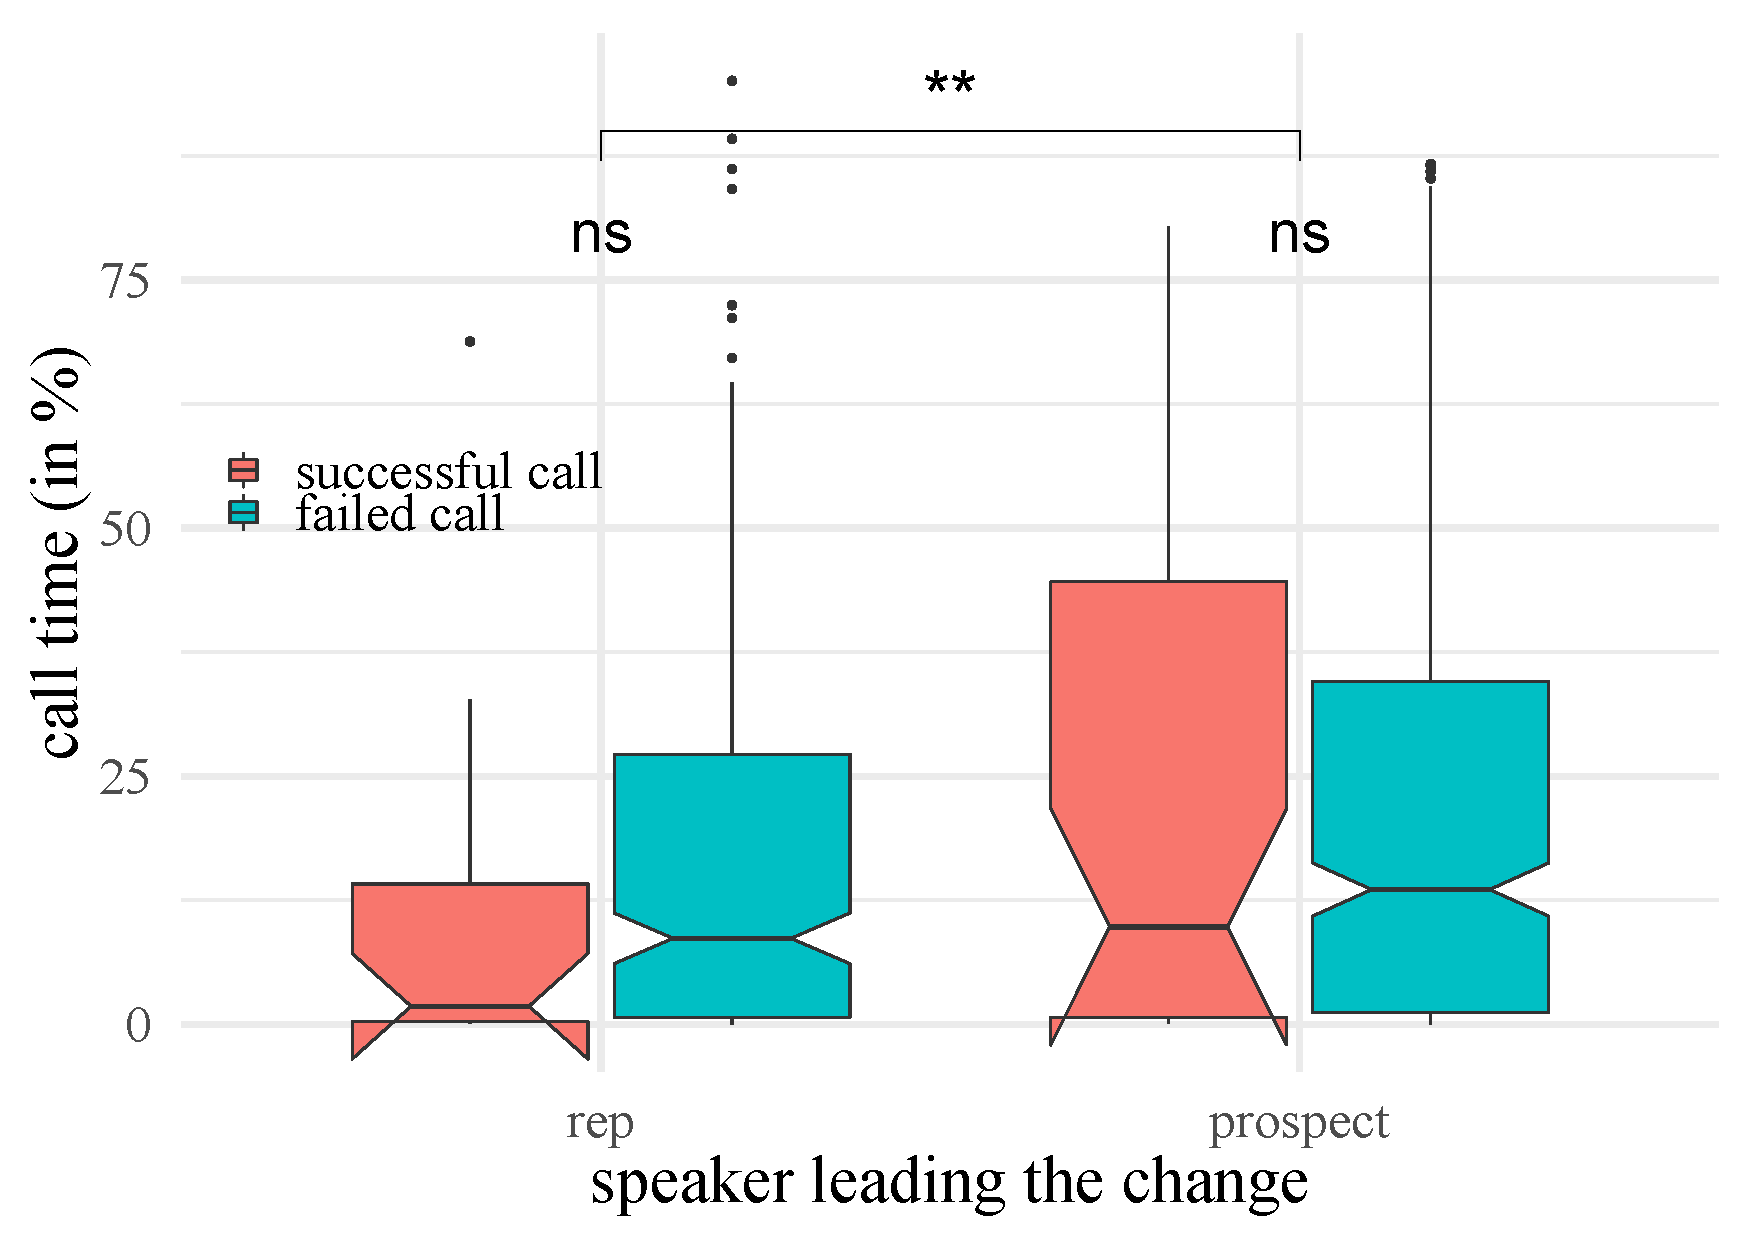
\includegraphics[width=\linewidth]{boxplot_ccf}
	\caption{Comparison between the time of the call in which the maximal \acl{cc} occurs.
		The x-axis groups the calls based on the speaker, and the fill color further separates the calls to successful and failed ones.
		The y-axis shows the normalized time (in percent) of the call, in which the maximal correlation was detected.
		The horizontal lines within the boxes represent the median,
		the notches stand for the \SI{95}{\percent} confident level of the median, the area inside the boxes include the \acf{iqr} of values, the vertical lines outside the boxes show the value within the third quartile + 1.5~$\protect\cdot$~\ac{iqr}, and the isolated dots are the outliers.
		The significance level based on a Wilcoxon test comparing the two groups and their subgroups is given above the boxes.}
	\label{fig:barplot_conv_leaders}
\end{figure}

\section{abstract}

\section{Introduction}
\label{sec:introduction}

Sales leaders have always aimed to reason why some of their representatives -- henceforth \emph{reps} or \emph{\acp{ae}} -- consistently attain or exceed their goals and others do not \citep{Kovac2017its}.
Yet, sales executives rely on data that is inherently flawed, as it is based on reports from sources such as \ac{crm} systems, leaving executives in the dark about the happenings at the front lines.
As a result, the reasons for losing or winning a deal often remain a riddle, making sales an art based on anecdotes rather than science \citep{Yohn2016best, Martin2017six}.
In his seminal book, \citet{Gladwell2006tipping} writes that \textquote[p.\ 83]{Part of what it means to have a persuasive personality is that you can draw others into your own rhythms and dictate the terms of the interaction}.
Supporting that, \citet{Orlob2018nine} found that star reps can make the prospect increase their speaking rate to match theirs, bringing the two sides closer with respect to this phonetic feature.

In this study, we focus on another phonetic feature, \ac{f0}.
This feature can also be interpreted and explained by people with little or no phonetic training, like \acp{ae}.
Furthermore, it can be easily controlled by speakers, making it a tangible tool for the \acp{ae} to exploit and improve their performance, as opposed to, e.g., more complex, acoustic features like \acp{mfcc} or changes in the \ac{ltas} that are often used in phonetic accommodation studies \citep{Levitan2011measuring,Borrie2019syncing}.

We use a large-scale corpus of real-world conversation, which takes the examination of phonetic accommodation out of the controlled, supervised experimental environment.
The conversations in the corpus are therefore more free-structured and flexible, as there are no instructions or defined tasks to perform, and presumably more authentic, since the interlocutors are driven solely by their own motivation to succeed and do not fill a temporary role as part of an experiment.

\Ac{crqa} \citep{Zbilut1998detecting}, a bivariate correlation technique, is used for the analysis (see \cref{subsec:crqa}).
This method finds instances where coordinates of two time series occur close to each other in some phase-space within a given radius.
Since \ac{crqa} can evaluate the degree to which the similarity of two time series changes over time, and can also determine the leading relationship between them, we find it suitable and informative for analyzing phonetic accommodation between two speakers.
A comprehensive overview of this method is presented by \citet{Wallot2018analyzing}, and the way it is used here is explained in \cref{subsec:crqa}.

The contribution of this work is therefore both in the methodology of measuring accommodation, and applying it in a practical situation.

%We hypothesize that since the prospect has agreed to meet for a demo and, in most cases, already heard about the proposed solution, the outcome of the call depends less on the prospect external condition and more on the personality of the sales person and her ability to build trust in the prospect.
%\todo{refer to where explain about dataset to justify the hypothesis.}

\subsection{Phonetic accommodation}
\label{subsec:phonetic_accommodation}

Depending on the situation, \ac{hhi} involves different levels of communication modality, such as facial expression, hand gestures, eye gaze, etc.
In this study, we concentrate on the phonetic level, as it is the main modality used in the sales calls dataset we analyze (see \cref{sec:dataset}).
It has been shown in various studies based on \ac{cat} \citep{Giles1991CAT,Gallois2015CAT} that humans naturally tend to change their speech behavior within a conversation based on the speech they hear from another human speaker \citep{Bailly2010speech,Babel2014novelty}.
Such mutual adjustment in \ac{hhi} also increases the success of the conversation \citep{Pickering2004behavioral} and affects the social distance between speakers \citep{Schweitzer2017social}.

The conversations in the large-scale corpus used here have an inherent structure and are longer than in typical experimental setups.
This encourages the use of \ac{crqa} to quantify the accommodation over the course of whole conversations to detect long-term relations and accommodation structures, instead of comparing two halves of the conversation or neighboring turns, as often done \citep{Levitan2013entrainment,Rahimi2018weighting}.

%Following that, we hypothesized that successful sales calls would show more distinct speech patterns and vocal accommodation behaviors than unsuccessful calls.

\subsection{Inside sales}
\label{subsec:inside_sales}

In recent years, many companies have adopted the concept of \emph{inside sales}, where \ac{b2b} sales are
done using web-based conferencing solutions, as opposed to face-to-face meetings with the clients.
Recent technological advancements allow automatic recording and transcription of inside sales calls, aggregating large-scale datasets.
These datasets include the audio of the calls and sometimes annotations such as the call success or the rating of the \ac{ae}.

Inside sales deals have a typical process:
first, a \ac{sdr} reaches out to a potential client (the \emph{prospect}) who has expressed interest in the company's product, which creates a \emph{lead}.
Subsequently, the \ac{sdr} shares basic details about the product and how it can help the prospect.
Finally, if the \ac{sdr} has managed to elicit initial interest, the lead turns into an \emph{opportunity}, and a demo call with a sales representative is scheduled.
Such demo calls are typically done using a web conferencing tool, such as Zoom\footnote{\url{https://zoom.us}} or GoToMeeting\footnote{\url{https://www.gotomeeting.com}}, which allows both sides to share their webcam and screen.

A relatively small dataset of such calls is analyzed in this work.
Since these calls were made as a first step after the prospect expressed interest in the company's product, it can be assumed that the behavior and verbal skills of the \ac{ae} will have a  larger weight in the success of the call than in calls that may fail solely because the product is of no interest to the prospect.

\section{Dataset}
\label{sec:dataset}

In this study we focus on calls of a single company.
The corpus for this study comprises only calls from an early stage of the sales opportunity that is also the first encounter between the participating \ac{ae} and the prospect.
Thus, these calls often include a description by the prospect of her business' history, challenges and plans, followed by a demo by the sales person that attempts to relate to those topics.
It is also important to note that although the \acp{ae} prepare for such calls, they are still spontaneous and in no way scripted.
With such set of calls, we can identify behavior patterns that are not related to the history between the two interlocutors or the content of previous conversations between them.
In some cases the prospect have already talked to an \ac{sdr} and/or communicated by email with the sales person.
However, to the best of our knowledge, this is the first voice call with the prospect.

The calls in this dataset were conducted using the Zoom platform, and were recorded automatically -- without any intervention from either side -- by Gong.io's system, which provides conversation intelligence services to said company.
Participants were notified of the recording, in compliance with relevant laws.
%The calls were then transcribed and diarized using an internal \ac{asr} system.

A single \ac{ae} and a single prospect participated in each call.
In total, 708 calls were used for analyses, each with a different customer company, with a total length of \SI{442}{\hour} (mean \SI{37.5}{\minute}, \ac{sd} \SI{15}{\minute}).
All of the calls are longer than 15 minutes, as many of the shorter calls were unsuccessful connection attempts.
Call recording started immediately following the first utterance by the prospect, and stopped when the meeting owner terminated it.
%This eliminates most issues related to one party waiting for the other party to join, and keeps only segments where both parties are present.
26 \acp{ae} (12 female) participated in the calls.
The vast majority of speakers on both sides were native speakers of American English.

We define a call as successful when a follow-up call under a more advanced stage is initiated or when an advancement in the opportunity is marked within one month.
Based on this criterion, 51 calls (\SI{7.2}{\percent}) were defined as successful, which is within the industry standard ratio for this kind of calls.
The average length of a failed call is \SI{37}{\minute} (\ac{sd} 15) and of a successful call, \SI{42}{\minute} (\ac{sd} 16.5).
A two-sample Wilcoxon test \cite{Wilcoxon1945individual} between failed and successful call duration yields a p-value of 0.04 with confidence level of \SI{95}{\percent}.
%Obviously, the labels of both criteria are noisy, as sales opportunities might be lost because of parameters more related to the fit between the offered product and the prospect's needs, the available budget of the prospect, the presence of competitors, legal issues that tamper the deal etc.

%We filtered out calls done by company personnel that are not sales people (for example, calls with \acp{sdr} that attempt to schedule demo meetings, or with Customer Success Managers who are often in charge of accompanying accounts after purchase).
%Sales people talked for X-X\% of the call (mean X\%, \ac{sd} X\%).
%The average duration of a monologue was X minutes and X seconds (\ac{sd} X minutes and X seconds) for sales people and prospect, respectively.
%The longest monologue of each participant in each call had a mean of X minutes and X seconds (\ac{sd} X and X seconds) for sales people and prospect, respectively.
%Automatic detection of questions based on the transcribed text showed that on average, the sales person asked X questions per minute (\ac{sd} X) compared with X (\ac{sd} X) for the prospect.
%We hypothesized that successful calls would show distinct patterns of phonetic convergence relative to unsuccessful calls.
%We measured the success of a call using two methods: (1) Based on the final outcome of the sales opportunity, being either won or lost.
%We call this method the "marriage" criterion, since it's similar to assessing a romantic date between two individuals as successful if it led to marriage and unsuccessful otherwise.

\section{Method}
\label{sec:method}

\subsection{Feature extraction}
\label{subsec:feature_extraction}

To increase temporal resolution, the audio signals were split into two-second slices.
Such fine-grained extraction makes the use of \ac{crqa} more elaborate, as it has more data points to consider (see \cref{subsec:crqa}).
Splitting the turns also creates equal, consecutive, and more comparable time units for an interaction without introducing artificial boundaries by dividing it into a predefined number of parts.
The slicing was done per turn, so that a slice contains only the speech of a single speaker.
Any remainder of a turn got a slice of its own.
When a speaker is not speaking (e.g., during the turn of the other interlocutor), it is assumed that the last produced value is maintained until the speech is renewed and a new value can be measured.
This way, no discontinuities are created and the same number of data points is extracted for both speakers, which creates a better temporal representation of the conversation.

Feature extraction was done sequentially for all the conversations using Praat\footnote{version 6.0.35} \citep{Boersma2001praat} scripts that first extracted the \ac{f0} value from the middle of each slice and then post-processed the output to acquire cleaner measures.

\section{Results}
\label{sec:results}

%In total, 708 calls were analyzed, from which 51 (\SI{7.2}{\percent}) were marked as successful as per the definition explained in \cref{sec:dataset}, which is an expected ratio in this kind of calls.
The \ac{crqa} yields 7 output values for each conversation:

\begin{description}[wide, nosep]
	\item[\Acf{rr}] the percentage of recurrent values between the two time series out of all the values.
	\item[Percentage determinism (DET)] the percentage of recurrences forming diagonal lines (with the minimum length being \SI{1}{\percent} of the series length).
	\item[number of lines (NRLINE)] The total number of lines formed by the recurrent values, i.e., the amount of accommodation between the two speakers that lasts longer than \SI{1}{\percent} of the time.
	Also referred to as \emph{sustained recurrence} by \citet{Borrie2019syncing}.
	\item[Maximal length (maxL)] the longest time period of recurrence, i.e., the longest time the speakers' speech remained close.
	\item[Average length (L)] the average time of recurrence.
	\item[Entropy (ENTR)] Shannon information entropy of diagonal line lengths longer than the minimum length.
	Describes the variability of the amount of accommodation between the two speakers across the whole call.
	\item[Normalized entropy (rENTR)] the entropy normalized by the number of lines formed by the recurrent values.
	This measure gives an idea how the speakers vary across multiple calls with different properties.
\end{description}

Since we compare multiple variables, Bonferroni correction was applied, so that the overall error rate across all variables is \num{0.05}.
Therefore, for a single comparison to be significant, it must be lower than $\alpha = 0.007$.
The non-parametric two-sample Wilcoxon test \citep{Wilcoxon1945individual} was used to determine the significance levels.
\cref{tab:crqa_results} shows a summary of means and p-values of these outputs between failed and successful calls.
The \ac{rr} mean value is about 10 in all groups, which proves to be a suitable goal for optimizing the parameters (see \cref{subsec:crqa}).
Significant differences between failed and successful calls were found for the values DET, NRLINE, and rENTR.
The first two, along with their higher means for the failed calls, indicate more time-synchronized convergence in the failed calls.
The latter is harder to interpret, especially due to the similar means for successful and failed calls.
It therefore seems that the behavior in both cases is evenly predicted, but differently across calls.
One possible factor influencing these behaviors is related to the interlocutor leading the convergence, rather than the fact that it occurs at all.

\begin{table}[t]
	\caption{P-values of the two-sample Wilcoxon test comparing the \ac{crqa} output values between calls with success/fail outcome and their respective mean values.
		Significant values based on the adjusted p-value are set in bold.}
	\label{tab:crqa_results}
	\begin{tabularx}{\linewidth}{XSSSS}
		\toprule
		& {\thead{\acs{rr}}} & {\thead{DET}} & {\thead{NRLINE}}	& {\thead{maxL}} \\
		\midrule
		p 				& 0.9		& \bfseries $\ll$ 0.001	& \bfseries $\ll$ 0.001	& 0.7  \\
		mean success	& 10.1		& 2.2					& 84.0					& 31.3 \\
		mean fail		& 10.0		& 5.9					& 174.0					& 32.9 \\
		
		%			p (leaders)		& 0.7		& 0.1						& 0.05						& 0.18\\
		%			mean \acsp{ae}	& 10.0		& 6.1						& 186.7						& 35.2\\
		%			mean prospect	& 10.1		& 5.4						& 154.4						& 31.2\\
		\midrule
		& {\thead{L}} 	& {\thead{ENTR}} 	& {\thead{rENTR}} 	& 						\\
		\midrule
		p 				& 0.07				& 0.1				& \bfseries 0.0058	& 	\\
		mean success	& 17.8				& 1.4				& 0.8				& 	\\
		mean fail		& 15.3				& 1.5				& 0.8				& 	\\
		
		%			p (leaders)		& 0.9		& 0.07		& 0.55					& {\qquad\qquad}\\
		%			mean \acsp{ae}	& 15.2		& 1.5		& 0.8					& {\qquad\qquad}\\
		%			mean prospect	& 15.7		& 1.4		& 0.8					& {\qquad\qquad}\\
		\bottomrule	
	\end{tabularx}
\end{table}

To shed more light on the role of a leading partner, we used \acl{cc} to determine which interlocutor leads the change in behavior.
As shown in \cref{fig:crqa_plot}, \ac{crqa} reports at which points in time the speakers were more inclined to be closer to each other.
As an extension, \acl{cc} finds the degree to which two time series are synchronized at different points in time.
For each such point, called \emph{lag}, the \acl{cc} function evaluates the correlation between the time series.
By iterating over a set of time points, the shift needed to make the time series maximally correlated can be found.
If this lag is positive, the first time series needs to be shifted forward to achieve maximal correlation, and vice versa.
In the context of convergence, \ac{cc} calculates the direction of the shift, which indicates which speaker leads the change.
The \acl{cc} function was not limited to a specific range of shifts, so that all possible lags were examined.
The lag associated with the maximal correlation -- and only it -- was used to determine the leader.
Since these calls have a typical structure, it is also interesting to see at which point of the conversation the maximal correlation occurs.
\cref{fig:barplot_conv_leaders} shows the time, in percentage, in which the maximal correlation occurred for \acp{ae} and prospects in successful and failed calls.
The difference between the lag position distribution of reps and prospects is significant, with a p-value of \num{0.0065} at $\alpha = 0.05$.
However, the differences between successful and failed calls within the leading speakers are not significant.
It is also evident that when the reps lead, they do so consistently at the very beginning of the conversation, all the more so in successful calls, whereas the prospects' lead varies much more and generally happens at a much later time.

\section{Discussion}
\label{discussion}

The results of the study show two sides of \ac{crqa} with respect to call success and role detection.

On the one hand, successful and failed calls could be distinguished by three of the \ac{crqa} output values.
Although based on \ac{hhi} studies it might be hypothesized that recurrence is more likely to occur in successful calls, the means of two of the three values suggest the opposite.
Surprisingly, this stands in line with some studies from sales research that show more \enquote{desperate} behavior from the rep side when a call seems to fail.
For example, over-emphasizing the deal's \ac{roi} -- with the hope that it will convince the prospect to buy -- often achieves the opposite effect \citep{Orlob2018roi}.
Another possible explanation is that reps give up their own lead in the call (see below) when a call is on the verge of failing, and instead let the prospect lead, either as a natural tendency or to give a better feeling.

On the other hand, utilizing \acl{cc} lags (i.e., how the recurrence needs to shift for the speakers to be maximally aligned) was useful for differentiating between the leader in the calls.
When \acp{ae} lead, they tend to do so at an earlier stage than prospects, especially in successful calls.
This, along with the \ac{crqa} results explained above, suggests that \acp{ae} do not necessarily always lead the conversation, but they know when to take advantage of it to improve their stance in calls.

Future research on this topic may go into three main directions.
First, deepening the aspect of the relationship between the \acp{ae} and the prospects by examining the mutual changes not only within single calls, but over the course of several meetings.
This could shed light on long-term changes and connect changes to the success of the deal.
Secondly, distinguishing between different \acp{ae} to find behaviors of sub-groups.
For example, sales persons with higher ratings (star reps) might be revealed to better exploit accommodation and trigger different behavior on the prospect side to increase their chance of closing a deal.
Lastly, different methods could be applied to predict the success of a call.
Specifically, machine learning methods that are good at capturing serial changes, such as recurrent neural networks, can be used to train such prediction models.
All of these direction can also be combined with more features to measure and more calls to analyze to reveal more consistent accommodation patterns.

\begin{figure}[t]
	\centering
	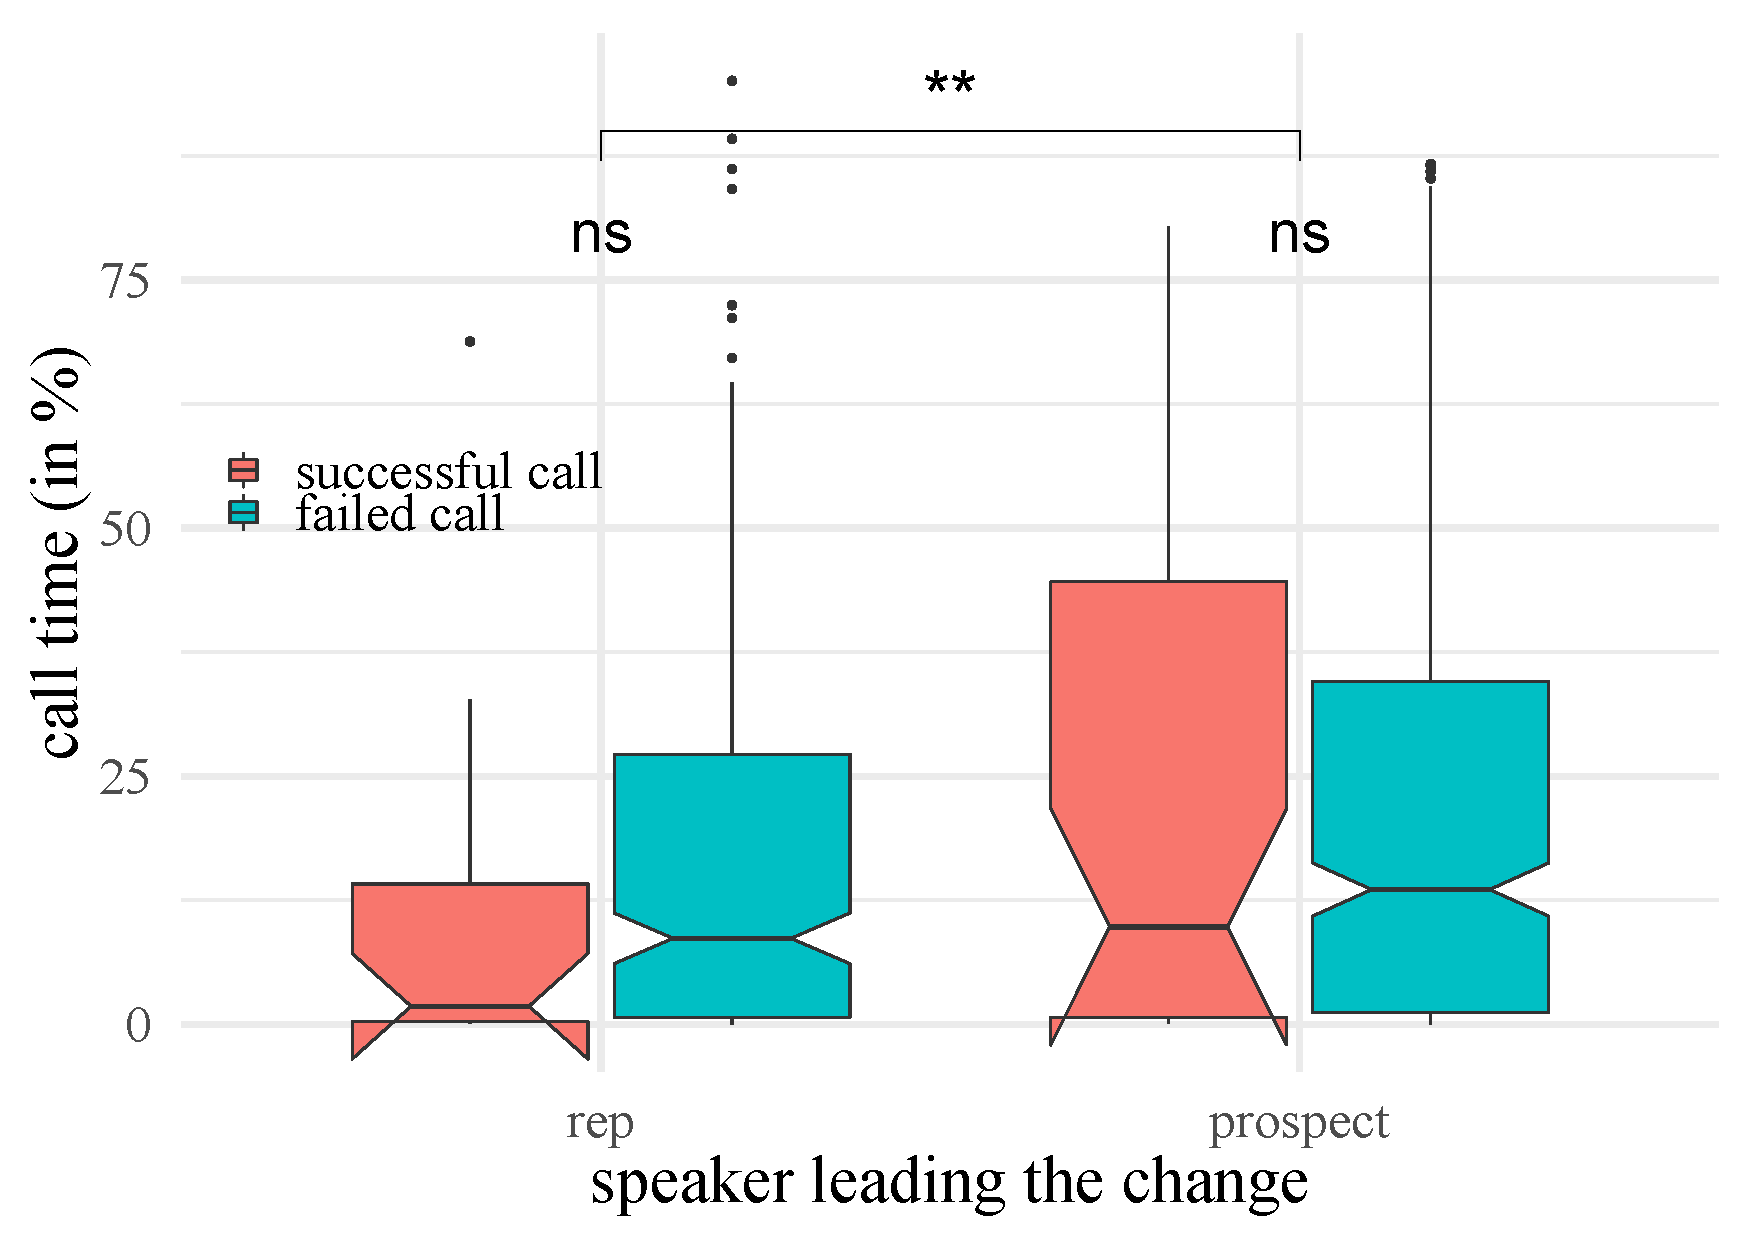
\includegraphics[width=\linewidth]{boxplot_ccf}
	\caption
		[Comparison between sales reps' and prospects' maximal \acl{cc} point in conversation for successful and failed calls.]
		{Comparison between the time of the call in which the maximal \acl{cc} occurs.
		The x-axis groups the calls based on the speaker, and the fill color further separates the calls to successful and failed ones.
		The y-axis points to the time in the call, in which the maximal correlation was detected.
		The horizontal lines within the boxes represent the median,
		%		the notches stand for the \SI{95}{\percent} confident level of the median, the area inside the boxes include the \acf{iqr} of values, the vertical lines outside the boxes show the value within the third quartile + 1.5~$\protect\cdot$~\ac{iqr}, and the isolated dots are the outliers.
		The significance level based on a Wilcoxon test comparing the two groups and their subgroups is given above the boxes.}
	\label{fig:barplot_conv_leaders}
	%	\todo[inline]{use logarithmic y-scale?}
\end{figure}


\section{Conclusion}
\label{sec:conclusion}

We have presented a study that examines phonetic accommodation in real-world sales calls.
The focus was on mutual proximity of \acl{f0} between sales persons and prospects to find both how close they are to each other in general across the call, and how quickly changes in proximity occur and by whom they are initiated.
This was done by \acf{crqa} and \aclp{cc}, which together provide various measures regarding recurrence between the speakers and who leads the other in terms of \acl{f0} changes.
A corpus of 708 calls was used for the analyses, which makes it possible to find more global, consistent effects that are not influenced by the design of a specific experimental setting.
The results show significant differences in some of the values between successful and failed calls, and significant differences between the leading behavior of sales persons and prospects.
These findings encourage further investigations, like looking for other predictors of successful calls and examining the influence of additional features and factors on the success of calls.

